%\section{RADS Framework and Algorithms}
\section{RADS Overview}
\label{sec:overview} 
%\noindent In this section we present an overview of RADS. Specifically, we discuss how RADS builds a linear classification model that differentiates between the ``positive" and the ``negative" classes as defined in the previous section, and we explain how RADS performs its real-time training and anomaly detection.

\noindent In this section we discuss how RADS builds a linear classification model that differentiates between the ``positive" and the ``negative" classes as defined in the previous section, and we explain how RADS performs its real-time training and anomaly detection.

%\text{One Class Classification (OCC).}
%RADS uses introduce the one class classification algorithm that is used as the linear classifier to differentiate between the ``positive" and the ``negative" classes defined in the previous section.
%\noindent We assume that the samples for the “negative” class are unknown, to differentiate between the two classes, RADS uses One Class Classification (OCC) algorithm that is proposed by Hempstalk et al. in~\cite{OCC:2008}. 
RADS aims to detect anomalies arising due to unknown DDoS and cryptomining attacks, traces of which are not previously recorded. Hence, we consider that the ``negative" class samples of the attacks are not available and RADS needs to build the classification model using the ``positive" class samples only. RADS achieves this by using the One Class Classification (OCC) algorithm that is proposed by Hempstalk et al. in~\cite{OCC:2008}. %The OCC algorithm does not require the ``negative" class samples. 
The algorithm first generates the artificial data (``negative" class) from a multi-variate normal distribution as estimated from the training data (``positive'' class) and, second, uses these artificial data as a second class in the construction of a binary class classification model, which is capable of classifying between the ``positive'' and the ``negative'' class. 
%Thus, this approach requires training with the data belonging to the ``normal" class in order to build the OCC models, which can classify between the `normal'' and the ``anomaly'' class. 
The classification is based on Bayes' Theorem\footnote{http://www.investopedia.com/terms/b/bayes-theorem.asp}.

\begin{figure}
  % {\epsfig{file = figures/RAIDS_framework, width = \textwidth, height=4cm}}
  \centering
     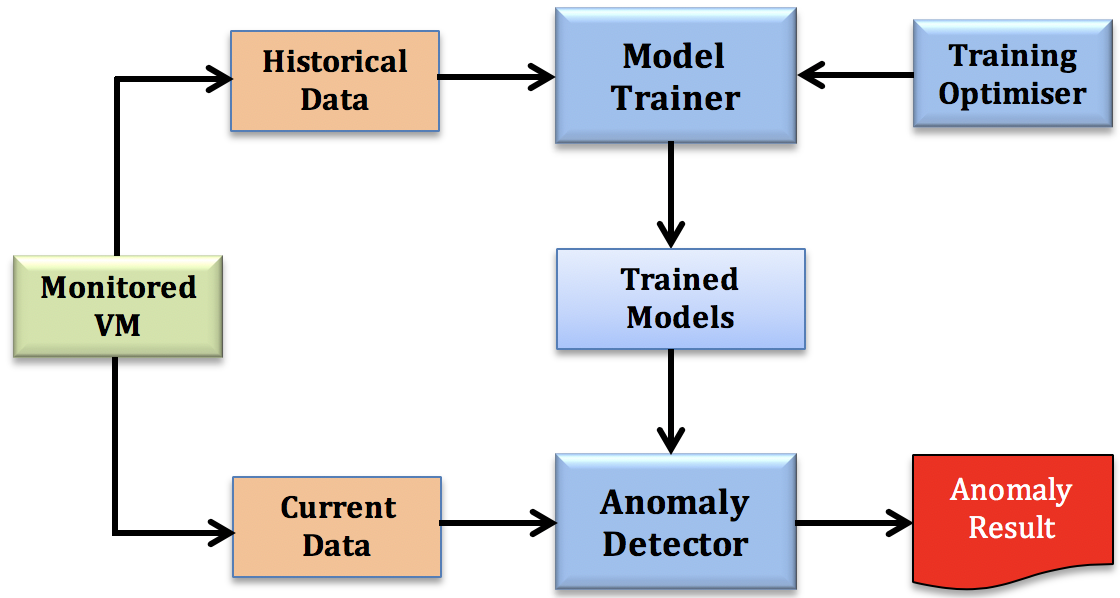
\includegraphics[width=0.7\textwidth]{figures/RADS_Overview}
   \caption{RADS overview}
  \label{fig:overview}
\end{figure}

%\textcolor{red}{Figure~\ref{fig:overview} presents an overview of RADS where we can see how RADS performs the training and the anomaly detection. 
Figure~\ref{fig:overview} depicts an overview of RADS. 
RADS runs the \textit{Model Trainer} to build or train the OCC models by using the ``positive" samples, i.e. the normal CPU utilisation or the network traffic data, which RADS collects from the hosted VMs in a Cloud data centre. Here it is important to note that RADS collects these training data assuming that the VMs are not affected by any DDoS or cryptomining attack. 
These training data are referred as the historical data as they are stored for a period of time. RADS uses the \textit{Training Optimiser} to decide the optimal amount of historical data to be used for the training of an OCC model. RADS runs the \textit{Anomaly Detector} to analyse the current data, i.e. the last one minute of CPU utilisation or the network traffic data by using the trained model. The model flags an anomaly whenever a VM's CPU or network usage pattern deviates significantly from its ``normal" pattern that is learned by the model. 
In both the training and the anomaly detection, RADS uses its window-based time series analysis as discussed in the previous section. 

%third phase - TRAINING OPTIMISER
\begin{algorithm}
\caption{Training Optimisation}
\label{raids_algorithm_training_optimiser}
%\algnewcommand\algorithmicheadingA{\underline{\textbf{{Data Pre-processing}}}}
\algnewcommand\algorithmicinput{\textbf{input:}}
\algnewcommand\algorithmicoutput{\textbf{output:}}
\algnewcommand\algorithmicabb{\textbf{abbreviation:}}
%\algnewcommand\HEADINGA{\item[\algorithmicheadingA]}
\algnewcommand\INPUT{\item[\algorithmicinput]}
\algnewcommand\OUTPUT{\item[\algorithmicoutput]}
\algnewcommand\ABB{\item[\algorithmicabb]}

\begin{algorithmic}[1]
%\algnewcommand\algorithmicheadingC{\underline{\textbf{{Intrusion Detection}}}}
%\algnewcommand\HEADINGC{\item[\algorithmicheadingC]}
%\HEADINGC
\INPUT $SPT$ - \textit{Stability Period Threshold}
%number of minutes to check OCC model's performance before declaring the model as stable
 \OUTPUT $TrainingStatus$ - first\_run/running/stopped/completed
 \ABB 
$ADR = Anomaly Detection Results$
\Statex
%\State $ModelStatus = ``stopped'" $
%\State RUN \textbf{Intrusion Detector} (Algorithm~\ref{raids_algorithm_intrusion_detection}) every 1 minute and store intrusion detection results in $IDR\_File$ 
%; IDR - Intrusion Detection Result
\For {\textbf{each} VM $vm_i$ \textbf{where} \textit{i=1,...,N}}
%\State $trainingStartTime=current\_time()$ \Comment time in minutes
\If {$TrainingStatus_i != ``completed"$} %\Comment execute training every 5 minutes 
%\State RUN algorithm \textbf{Training Data Pre-processing} \Comment execute in every 5 minutes 
%\State RUN \textbf{Model Trainer} (Algorithm~\ref{raids_algorithm_model_training}) % every 5 minute
\If {($TrainingStatus_i = ``first\_run"$ OR \textbf{ADR} contains ``anomaly")} 
\State RUN \textbf{Model Trainer}
\State $TrainingStatus_i = ``running"$
\State $stabilityPeriod_i = 0$
\State $break$
\Else 
%\State INCREMENT stabilityPeriod BY 5 minutes 
\State $stabilityPeriod_i = stabilityPeriod_i + 5$
\EndIf
\If {$(stabilityPeriod_i = SPT)$}
\State $TrainingStatus_i = ``completed"$
\Else
\State $TrainingStatus_i = ``stopped"$
\EndIf
\State CLEAR $ADR\_File$
\EndIf
\EndFor
%\State \textbf{return} $ModelStatus$ \newline
%\State \textbf{Store} $ModelStatus$ in  \textbf{Model Storage} \newline
\end{algorithmic}
\end{algorithm}
%\vfill


%third phase - INTRUSION DETECTION
\begin{algorithm}
\caption{Anomaly Detection}
\label{raids_algorithm_intrusion_detection}
%\algnewcommand\algorithmicheadingA{\underline{\textbf{{Data Pre-processing}}}}
\algnewcommand\algorithmicinput{\textbf{input:}}
\algnewcommand\algorithmicoutput{\textbf{output:}}
\algnewcommand\algorithmicabb{\textbf{abbreviation:}}
%\algnewcommand\HEADINGA{\item[\algorithmicheadingA]}
\algnewcommand\INPUT{\item[\algorithmicinput]}
\algnewcommand\OUTPUT{\item[\algorithmicoutput]}
\algnewcommand\ABB{\item[\algorithmicabb]}

\begin{algorithmic}[1]
%\algnewcommand\algorithmicheadingC{\underline{\textbf{{Intrusion Detection}}}}
%\algnewcommand\HEADINGC{\item[\algorithmicheadingC]}
%\HEADINGC
%\INPUT $INN_{testing}$ - N normalised input instances for testing (one for each VM); $M$ - set of N trained OCC models
\INPUT $CurrentData$ - last one minute of CPU utilisation or network traffic data for each VM; $M$ - set of trained OCC models (one for each VM)
%\OUTPUT $INN_{testing}$ - normalised input instance for testing ; total N instances for N Cloud applications
 \OUTPUT $ADR$ - Anomaly Detection Result (one for each VM)
\Statex
\For {\textbf{each} VM $vm_i$ \textbf{where} \textit{i=1,...,N}}
\State $classificationResult_i=M_i.classify(CurrentData_i)$
 \If {$(classificationResult_i = ``positive")$}
\State $ADR_i= ``normal"$
\Else %If {($classificaitonResult_i = 1$)}
\State $ADR_i= ``anomaly"$
\EndIf
\EndFor
%\State \textbf{Store} ADR in \textbf{Detection Results} \newline
%\State \textbf{return} $IDR$ \newline
\end{algorithmic}
\end{algorithm}
%\vfill

\begin{figure*}
  % {\epsfig{file = figures/RAIDS_framework, width = \textwidth, height=4cm}}
  \centering
     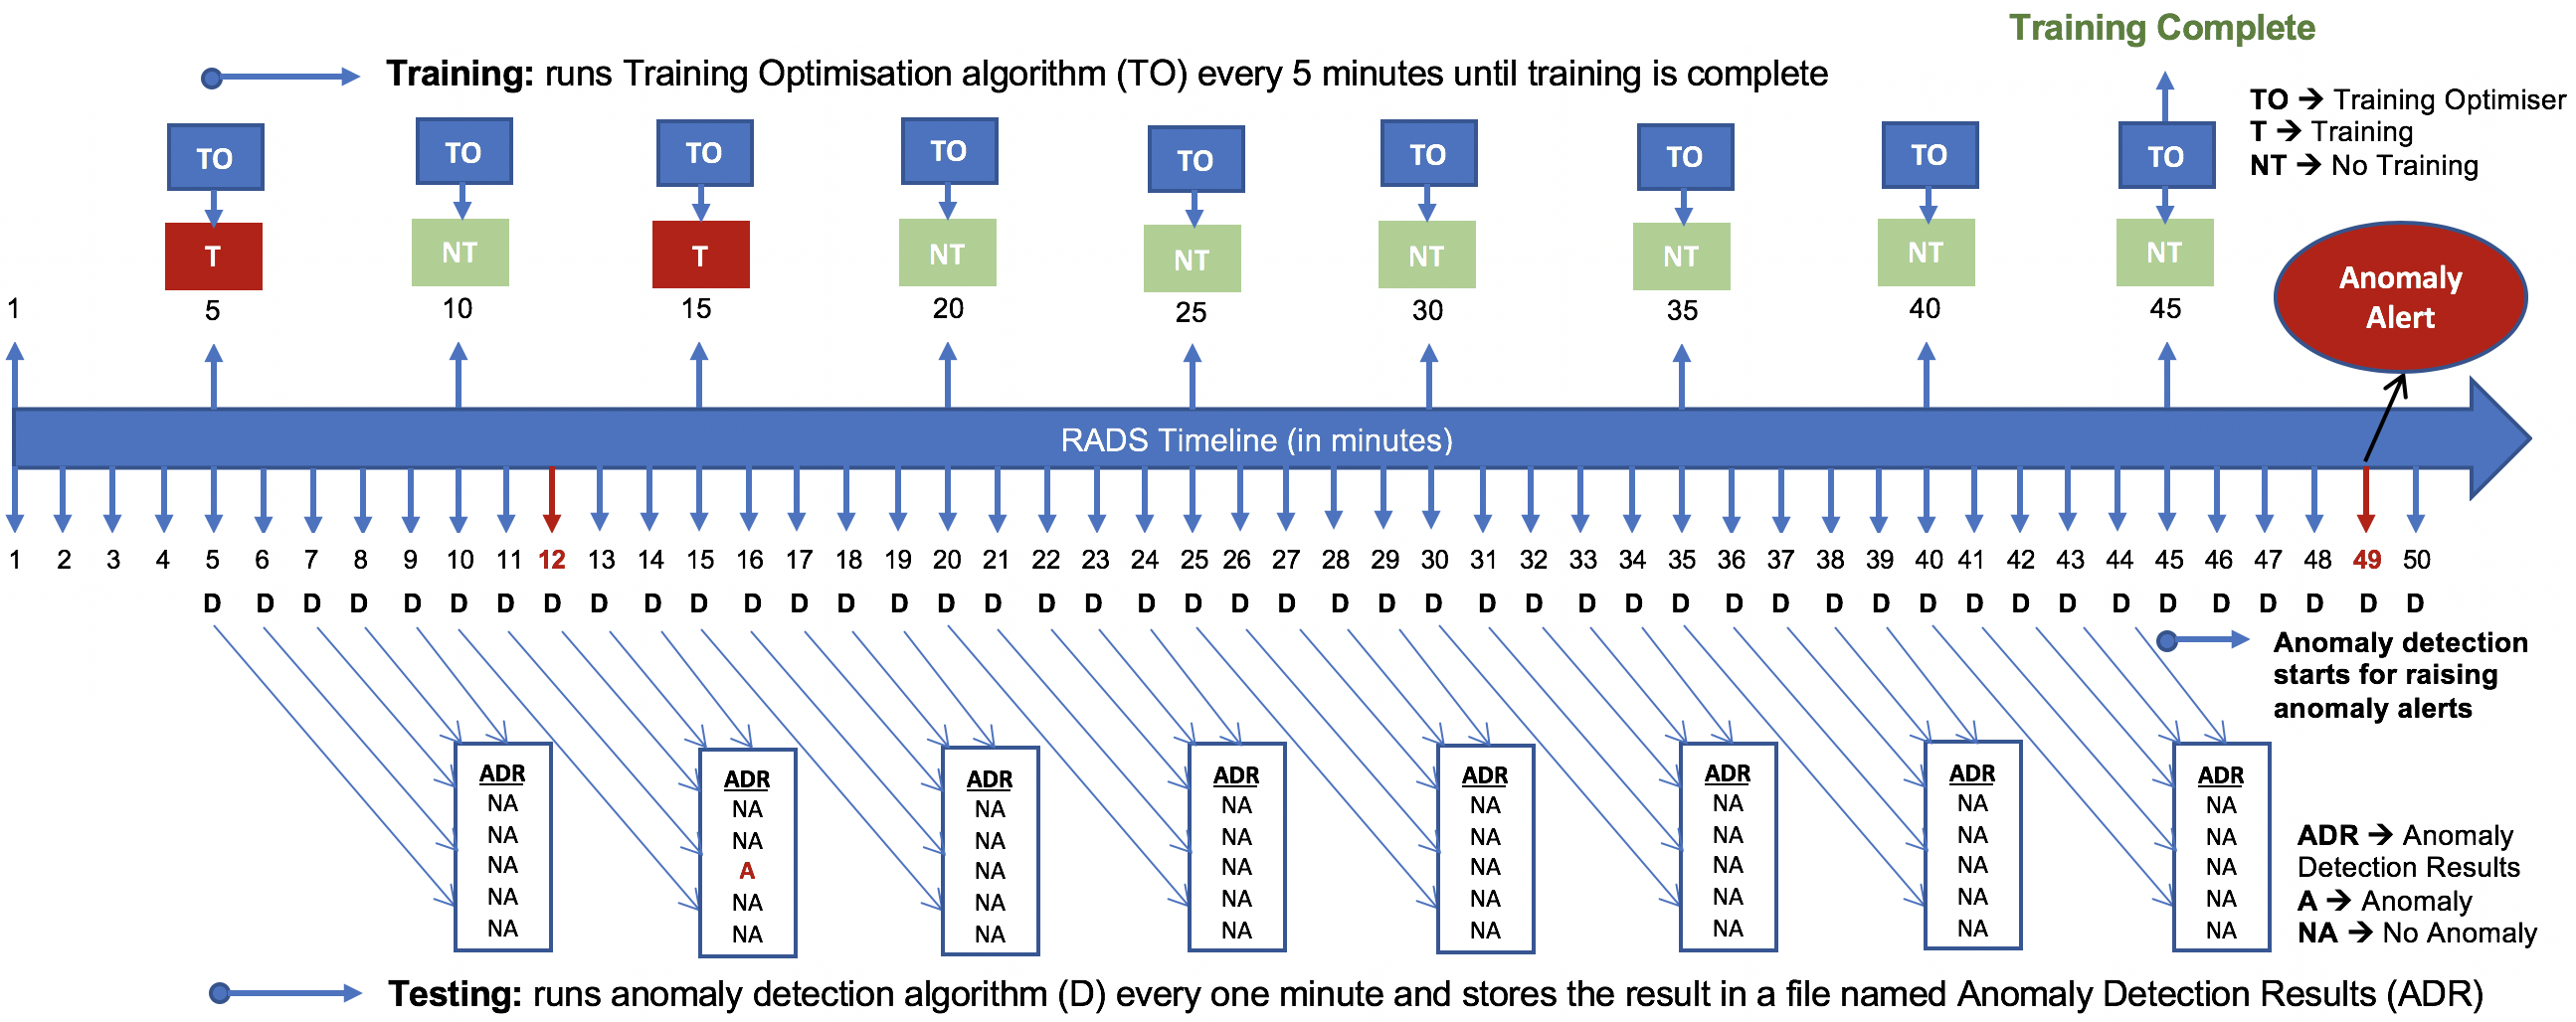
\includegraphics[width=1\textwidth]{figures/RADS_Timeline}
   \caption{RADS  real-time training and anomaly detection}
  \label{fig:timeline}
\end{figure*}
%\vfill

We explain the real-time training and anomaly detection of RADS using a timeline as depicted in Figure~\ref{fig:timeline}. Specifically, we present the timeline of 50 minutes of RADS activity while performing training and detecting anomalies in real-time for a specific VM. We set up the behaviour of the VM artificially where the VM is behaving normally at all times except for minutes 12 and 49 where the VM experiences a genuine spike and an anomaly, respectively. For the first five minutes, RADS remain idle in order to accumulate data points to work with. At the end of 5\textsuperscript{th} minute, RADS starts its training which runs the training optimisation algorithm (TO) (Algorithm~\ref{raids_algorithm_training_optimiser}) every 5 minutes and starts its testing which runs the anomaly detection algorithm (D) (Algorithm~\ref{raids_algorithm_intrusion_detection}) every 1 minute. 
%The time intervals for running TO and D are decided based on our experimental findings. 
When the TO runs for the first time (at the end of 5\textsuperscript{th} minute), it performs the training to build the OCC model for the first time. In the later occasions, the TO evaluates the performance of the trained model by checking whether the model is identifying the VM's behaviour accurately without any false positive. 
This checking is performed by analysing the last five minutes of the anomaly detection results (ADR) obtained from D.
%; the results are stored in a file named Anomaly Detection Results (ADR). 
%This checking is performed by analysing the last five minutes of the results obtained from D; the results are stored in a file named Anomaly Detection Results (ADR). 
We assume that the VM is anomaly-free during the runtime of TO. 
Therefore, if the ADR contains ``anomaly" or ``A", that means that there is an anomaly falsely flagged by the trained model and the model needs to be trained again; in the timeline we can see that at the end of 15\textsuperscript{th} minute the training is performed again due to the occurrence of a false positive generated by the genuine spike at 12\textsuperscript{th} minute.
If the ADR does not contain ``anomaly" or ``A", that means that the model is correctly identifying the VM's behaviour and the model does not need further training; in the timeline we can see that at the end of 10\textsuperscript{th}, 20\textsuperscript{th}, 25\textsuperscript{th}, 30\textsuperscript{th}, 35\textsuperscript{th}, 40\textsuperscript{th}, and 45\textsuperscript{th} minutes the training is stopped. 

The period of time for which the model correctly identifies the ``normal" behaviour, is considered as the stability period for the model. The stability period is incremented with each correct identification by the model (e.g. in the timeline while moving from minute 15 to 45, the stability period is incremented to 30 minutes). Whenever the stability period reaches its threshold value, the TO declares that the training is complete; in the timeline we can see that at the end of 45\textsuperscript{th} minute as we set the threshold value to 30 minutes, which is based on the behaviour of the workloads executed in our testbed. 
However, the threshold for the stability period needs to be adjusted for different VMs based on their workload behaviour; a Cloud data centre may do this based on the type of the instances. 
Once the training is complete, RADS starts its anomaly detection for raising anomaly alerts; in the timeline we can see how RADS raises an anomaly alert at the 49\textsuperscript{th} minute due to the anomalous behaviour of the VM.

%In our experiments, we decided to set the stability period threshold to be 30 minutes, which is based on the behaviour of the workloads executed in our testbed (lab-based Cloud data centre). 
%}
%In both the training and the anomaly detection, RADS uses its window-based time series analysis as discussed in the previous section. }

%The module runs every one minute and stores the detection results in the \textbf{Detection Results}. The storing of the detection results is for the purpose of dynamically deciding the training duration for each OCC model; which allows performing real-time training of the OCC models where the models get updated in real-time at regular intervals until they start performing accurately. 
%To achieve this, RADS applies a heuristic that dynamically decides the training duration for each OCC model.
%As discussed in Section~\ref{sec:introduction}, due to the dynamic nature of Cloud applications, it is required to dynamically decide the training duration for the behavioural models based on the behaviour of the applications. Static models, which are built with fixed training duration may result in low detection accuracy due to model overfitting or underfitting issues.
%The storing of the detection results for a VM continues while the model status for that VM is not ``completed", which means until the model is completely trained for that VM. If the model is completely trained for a VM and an ``anomaly" is detected, RADS flags an anomaly alarm. 


%Finally, we illustrate how RADS dynamically decides the training duration for each OCC model using the \textit{Training Optimiser algorithm} (Algorithm~\ref{raids_algorithm_training_optimiser}).
%This is an important feature of RADS, which can train the OCC models with appropriate set of training data in order to reduce the effect of model overfitting or underfitting. This can also help in dealing with the behavioural changes in workload over time (referred to as concept drift).
%one important feature of the \textbf{Model Trainer} module, which is its ability to dynamically decide the training duration. This feature helps to train the OCC models with appropriate set of training data to reduce the effect of model overfitting or underfitting. 
%As discussed in Section~\ref{sec:introduction}, due to the dynamic nature of Cloud applications, it is required to dynamically decide the training duration for the behavioural models based on the behaviour of the applications. Static models, which are built with fixed training duration may result in low detection accuracy due to model overfitting or underfitting issues.
%The algorithm runs every five minutes and decides whether the training of the OCC model for a particular VM needs to be run or stopped. This decision is based on the real-time performance of the models, which is evaluated by checking whether the model for a VM is identifying the VM's ``normal" resource usage pattern accurately without any false positive for a significant period of time. This checking is performed by analysing the last five minutes of the anomaly detection results (ADR) for that VM. If the ADR contain ``anomaly", that means that there is an anomaly falsely flagged by the trained model and the model for the VM needs to be trained again. Hence, the model training continues for that VM. If the ADR do not contain ``anomaly", that means that the model is correctly identifying the VM's ``normal" resource usage pattern and the model does not need further training. The period of time for which the model correctly identifies the ``normal" usage pattern, is considered as the stability period for the model. The stability period is incremented with each correct identification by the model. Whenever the stability period for a particular model reaches the threshold value set for the stability period, the module declares that the training is complete for that model and updates the model status as ``completed". The threshold for the stability period needs to be decided based on the VMs' workload behaviour; a Cloud data centre may take this decision based on the type of the instances. In our experiments, we decided to set the stability period threshold to be 30 minutes, which is based on the behaviour of the workloads executed in our testbed (lab-based Cloud data centre). 
%We present the algorithm designed for dynamically deciding the training duration in Algorithm~\ref{raids_algorithm_training_optimiser}.

